\documentclass{report}
\usepackage{longtable}
\usepackage{adjustbox}
\usepackage[intlimits]{amsmath}
\usepackage{mathtools}
\usepackage{nonfloat}
\usepackage{amsmath}
\usepackage{verbatim}
\usepackage{amsthm}
\usepackage{setspace}
\usepackage[paperwidth=16cm,paperheight=24cm]{geometry}
\usepackage[a4,frame,center]{crop}
%\graphicspath{{/home/abhishek/Desktop/"Text Classification"/Report/figures/}}
\graphicspath{{./figures/}}
\usepackage{lipsum}% dummy text
\usepackage[titles]{tocloft}
\usepackage{amssymb}
\setlength\cftbeforechapskip{100pt}
\renewcommand\cftfigafterpnum{\vskip10pt\par}
\renewcommand\cfttabafterpnum{\vskip10pt\par}
\usepackage[superscript,biblabel]{cite}
\usepackage{tocloft,lipsum,pgffor,sectsty}

\setcounter{tocdepth}{4}% Include up to \subsubsection in ToC




% Font changes to ToC content of sectional units
\renewcommand{\cftpartfont}{\normalfont\sffamily\bfseries}% \part font in ToC
\renewcommand{\cftchapfont}{\normalfont\large\itshape}    % \chapter font in ToC
\renewcommand{\cftsecfont}{\normalfont\slshape}           % \section font in ToC
\renewcommand{\cftsubsecfont}{\normalfont\itshape}        % \subsection font in ToC
\renewcommand{\cftsubsubsecfont}{\normalfont\small}       % \subsubsection font in ToC

% Font changes to document content of sectional units
\renewcommand{\partfont}{\normalfont\HUGE\bfseries}
\renewcommand{\chapterfont}{\normalfont\HUGE\bfseries}
\renewcommand{\sectionfont}{\normalfont\Huge\bfseries}
\renewcommand{\subsectionfont}{\normalfont\Huge\bfseries}

\usepackage{url}
\usepackage{enumitem}
\usepackage{chngcntr}
\usepackage[svgnames]{xcolor}
\usepackage{pgfplotstable}
\usepackage{pgfplotstable,booktabs}
\usepackage{csvsimple}
\usepackage{multicol}
\usepackage[pdfpagemode=FullScreen, colorlinks=true]{hyperref} 
\usepackage{hyperref}
\hypersetup{%
  colorlinks = false,
  linkcolor  = black
}
\usepackage{graphicx}
\usepackage{subcaption}
\usepackage{filecontents}
\newcommand{\plogo}{\fbox{$\mathcal{PL}$}}
\usepackage[utf8]{inputenc}
\usepackage[T1]{fontenc}
\usepackage{fouriernc}
\usepackage[utf8]{inputenc}
\usepackage{titlesec}
%\usepackage{etoolbox}
%\makeatletter
%\patchcmd{\ttlh@hang}{\parindent\z@}{\parindent\z@\leavevmode}{}{}
%\patchcmd{\ttlh@hang}{\noindent}{}{}{}
%\makeatother
\usepackage{titletoc}
\usepackage[figurename=Fig - ]{caption}
\captionsetup[table]{skip=20pt}
\captionsetup[figure]{skip=20pt}
\usepackage[tablename=Table - ]{caption}


\usepackage{setspace}

\usepackage{titlesec}
\titleformat{\chapter}[display]
  {\normalfont\Huge\bfseries}{}{0pt}{}

\usepackage{geometry}
 \geometry{
 a4paper,
 tmargin=20mm,
 bmargin=15mm,
 left=20mm,
 right=20mm,
 top=20mm,
 }

\renewcommand\thesection{\arabic{section}}
\titlecontents{chapter}[1.05em]{\bigskip}%
{\contentslabel[\MakeUppercase{\romannumeral\thecontentslabel}]{1em}\enspace\textsc}%numbered\contentslabel
{\hspace*{-1em}\textsc}%numberless
{\hfill\contentspage}%
%
\titlecontents{section}[1.6em]{\bigskip}%
{\thecontentslabel.\enspace}%numbered
{}%numberless
{\titlerule*[1pc]{.}\contentspage}%

\setcounter{tocdepth}{6}

\usepackage{lipsum}

\newcommand\myfigure[1]{%
\medskip\noindent\begin{minipage}{\columnwidth}
\centering%
#1%
%figure,caption, and label go here
\end{minipage}\medskip}




\newenvironment{changemargin}[1]{%
\item[]}{\end{list}}
\setlength{\columnsep}{0cm}


\titlespacing*{\chapter}{0pt}{0pt}{20pt}

\renewcommand{\bibname}{References}

\usepackage{makeidx}
\makeindex

\begin{document} 

\begin{titlepage}
	\centering
	
\includegraphics[width=4cm]{logo.png}\\[.5cm]
	{\scshape\LARGE Indian Institute of \\Information Technology, Allahabad \par}
	\vspace{1cm}
	\rule{\textwidth}{2pt}	
	%\vspace{2pt}\vspace{-\baselineskip}
	%\rule{\textwidth}{0.4pt}
	\vspace{0.1\textheight}
		
	\textcolor{Red}{ 
		{\fontsize{35}{42}\selectfont DeliveryMates}\\[0.5\baselineskip]
	}
	
	\vspace{0.185\textheight} 
	
	\rule{0.3\textwidth}{0.4pt} 
	\begin{multicols}{3} 
	\textcolor{Blue}{
		\begin{flushleft} 
		{\large Ayush Agnihotri}\\[5pt] 
		{\large Nidheesh Pandey}\\[5pt]
		{\large Abhishek Pasi}\\[5pt]
		\end{flushleft}
		}
		\columnbreak
		 
	\textcolor{Blue}{
		\begin{flushleft} 
		{\large IIM2015004}\\[5pt] 
		{\large IIM2015501}\\[5pt]
		{\large ICM2015002}\\[5pt]
		\end{flushleft}
		}
		\columnbreak

	\textcolor{Green}{
		\begin{flushright}
		{\Large \textsc{Under supervision}}\\
		{\large of}\\
		{\Large \textsc{\textbf{Dr. Jagpreet Singh}}}
		\end{flushright}
		}
	\end{multicols}
	\vspace{0.065\textheight} 
	
\hfill


	\rule{\textwidth}{0.4pt} % Thin horizontal rule
	
	\vspace{2pt}\vspace{-\baselineskip} % Whitespace between rules
	
	\rule{\textwidth}{2pt} % Thick horizontal rule
	
\end{titlepage}
\pagebreak

%---------------------------------------------------------------------------------------------------

{\chapter*{ \quad \quad \quad \quad \quad \quad  \Huge \scshape \underline {Declaration} }
\vspace{2.0cm}
\begin{spacing}{0.3}
\fontsize{17}{68}\selectfont\linespread{10} {We hereby declare that the work presented in this project report entitled \textbf{``DeliveryMates''},  submitted towards progress of summer project report of Dual Degree(IT) at \textbf{Indian Institute of Information Technology, Allahabad}, is an authenticated record of our original work carried out from \textbf{May 2018} to \textbf{present} under the guidance of \textbf{Dr. Jagpreet Singh}. Due acknowledgements have been made in the text to all other material used. The project was done in full compliance with the requirements and constraints of the prescribed curriculum.}
\end{spacing}
\vspace{5cm}
\Large
\noindent \textbf{Signature Of Supervisor:}\\
\rule[0.5em]{25em}{0.5pt} % This prints a line for the signature
\vspace{1cm}\\
\noindent \textbf{Date:}\\
\rule[0.5em]{25em}{0.5pt}\\ % This prints a line to write the date
\vspace{1cm}\\
\noindent \textbf{Signature Of Students:}\\
\rule[0.5em]{12em}{0.5pt} % This prints a line for the signature
\vspace{1.5cm}\\

}


%----------------------------------------------------------------------------------------
%---------s-------------------------------------------------------------------------------
%	LIST OF CONTENTS/FIGURES/TABLES PAGES
%----------------------------------------------------------------------------------------

\pagenumbering{arabic}
{ \doublespacing
\pagenumbering{Roman}
\tableofcontents % Prints the main table of contents

\addtocontents{toc}{~\hfill\textbf{Page}\par}
\pagebreak
\listoffigures % Prints the list of figures
\pagebreak
\listoftables % Prints the list of tables
\pagebreak

}

%-----------------------------------------------------------------------------------------
\title{\Huge  DeliveryMates\linebreak}
\date{}
\maketitle
\setlength{\columnsep}{0.7cm}
\pagenumbering{arabic}
%\begin{multicols}{1}
\chapter{Abstract}
\par \Large \textit {The main aim of this report is to define an approach to implement cross-domain sentiment analysis. Although traditional classification algorithms can be used to train sentiment classifiers from manually labeled text data but the labeling work can be time-consuming and expensive. Moreover,If we directly apply a classifier trained in one domain to other domains, the performance will be very low due to the differences between these domains.Therefore we are using a Transfer Learning approach for classification of Cross Domain datasets.\\
\linebreak
In our approach, we took datasets from two different but related domains,and used one of them  as source and other as target domain dataset. We extract the features from both of these datasets and classify the extracted features into domain independent features (pivot features) and domain specific features. We used bipartite graph representation between domain independent and domain specific features to find co-ocurrence  between these two types of features.Spectral Clustering algorithm is then applied to cluster the domain specific features around closely related pivot features. This reduces the gap between domain-specific words of the two domains.Now we have a new augmented set of features containing all the features of source domain + the newly found clustered features. This new feature representation is then used to train the sentiment classifier, to classify the target domain accurately.\\
\linebreak
Since we have labeled dataset in target domain, so we can test the accuracy of our model by direct comparison. Comparison with other cross domain sentiment analysis algorithms and various optimisations techniques to improve the accuracy of the model will be added in future version of this report
}

%---------------------------------------------------------------------

\chapter{Introduction}

\par \Large The world is getting flooded by textual data everyday. It is very important to extract infromation from this data for better understanding of the world. These data includes product reviews, blogs, public opinions, stock trends etc. The informations hidden in these data is used by bussiness firms, govt. agencies to formulate the policies and future plans. Inorder to extract this important inforamtion we need labeled datasets. Most of the textual data present today is unlabeled which makes it highly difficult to analyze them. \\

\par Earlier works in sentiment analysis involved various supervised learning algortihms. For using supervised learning methodologies we require labeled datasets. Labeling a dataset manually is time consuming and expensive. Also the earlier models were domain specific ( i.e. when a classifier trained in one domain is applied in other domains, then it performs poorly). So, there does not exist a general classifier which can be used for sentiment analysis in multiple domains.  \\

\par In this report we would like to present a model which will do Sentiment Analysis on various domains and for unlabeled datasets. It does this by learning the knowledge from a labeled dataset and transfering the learnt knowledge. We took a labeled dataset as source domain inorder to train our classifier for target domain.\\

\par The main algorithm we are implementing is Spectral Feature Alignment (SFA) algorithm which helped us to represent cross domain data in a combined way to form as a new set of features. SFA does this by clustering domain specific features around domain independent features depending upon the co-ocurrence between the domain specific and domain independent features. These features are represented uses bipartitte graph.\\

\par The concept is that,
\begin{enumerate}[label=\arabic*.]
\item if two domain-specific features are connected to many common domain-independent features, then they tend to be very related and will be aligned to a same cluster with high probability,
\item  if two domain-independent features are connected to many common domain-specific features, then they tend to be very related and will be aligned to a same cluster with high probability.
\end{enumerate}
We have implemented this using Spectral Clustering (based on graph spectral theory) on the bi-partite graph to co-align domain-specific and domain-independent words into a set of feature-clusters. The clusters helps us to reduce the degree of mismatch between domain specific features of both domains. So, our final feature set is based on this combined cluster representation.
Then our classsfier is trained on this new feature set which is able to do cross domain sentiment analysis with greater accuracy level than traditional methods.

We'll optimise the accuracy of our classifier model using SFA and do the corresponding experiments .

%---------------------------------------------------------------------------------------------------

\chapter{Literature survey}

\begin{enumerate}[label=\alph*).]
\item \textbf{Jialin} et. al.\cite{Pan:2010:CSC:1772690.1772767} focuses on how to do sentiment analysis on cross domains using SFA algorithm. Here first domain-specific \& domain-independent features are extracted \& unified into clusters using Spectral Feature Clustering. This feature set is then used by classifier for cross-domain sentiment analysis.
\item \textbf{Lin} et. al.\cite{Lin:2014:EEM:2661829.2662071} proposed a general ensemble technique which takes into account model application, model weight \& strategies for selecting most related models with respect to a target node. Here two strategies, cosine function and taxonomy-based regression model (TBRM) are proposed to select most related models.
\item \textbf{WuFangzhao} et. al.\cite{WU201726} proposes a novel approach to train domain-specific sentiment classifiers by fusing the sentiment knowledge from multiple sources. The \(1^{st}\) source is sentiment lexicons , \(2^{nd}\) is sentiment classifier of multiple domain, \(3^{rd}\) unlabeled data in target domain, \(4^{th}\) is labeled data in target domain. It alsoproposes a unified framework to fuse these four kinds of \& train domain-specific sentiment classifier for target domain.
\item \textbf{Nelakurthi} et. al.\cite{doi:10.1137/1.9781611974973.53} addresses this problem by explicitly modeling the human factor related to sentiment classification. To this end, he proposed a new graph-based approach named U-Cross, which models the relatedness of different domains via both the shared users and keywords. It is non-parametric and semi-supervised in nature.
\item \textbf{Fangzhao Wu} et. al.\cite{Wu:2016:SDA:2983323.2983851} gave a new sentiment domain adaptation approach by adapting the sentiment knowledge in general-purpose sentiment lexicons to a specific domain is proposed. Moreover it also proposes a unified framework to incorporate these different kinds of sentiment knowledge and learn an accurate domain-specific sentiment classifier for target domain.
\end{enumerate}


%------------------------------------------------------------------------------------------------------------------

\chapter{Problem Statement}
\section{Problem Definition :}
Given two domains \(D_{src}\) and \(D_{tar}\) , where \(D_{src}\) and \(D_{tar}\) are referred to as a source domain and a target domain respectively, suppose we have a set of labeled training sentiment data \(\mathcal{D}_{src}\) = \{(\(x_{src i}\)  , \(y_{src i} )\}_{i=1}^{n_{src}}\) in \(D_{src}\) , and some unlabeled sentiment data tar , \(\mathcal{D}_{tar}\) = \{\(x_{tar j} \}_{j=1}^{n_{tar}}\) in \(D_{tar}\) . The task of cross-domains sentiment classification is to learn an accurate classifier to predict the polarity of unseen sentiment data from \(D_{tar}\) .\\
\linebreak
\section{Some definitions :}
\subsection{Definition 1:}
\textbf{Domain :-}A domain D denotes a semantic concept.\\
\textbf{Example :-} different types of products like toys, electronics, books, kitchen can be regarded as domains.\\
\subsection{Definition 2:}
\textbf{Sentiment :-} In Context of a given domain D, Sentiment data is a text document which conveys some opinion. 

%---------------------------------------------------------------------------------------------------
\chapter*{Methodology Flow Diagram}
\vspace{100pt}
\begin{figure}[!h]
	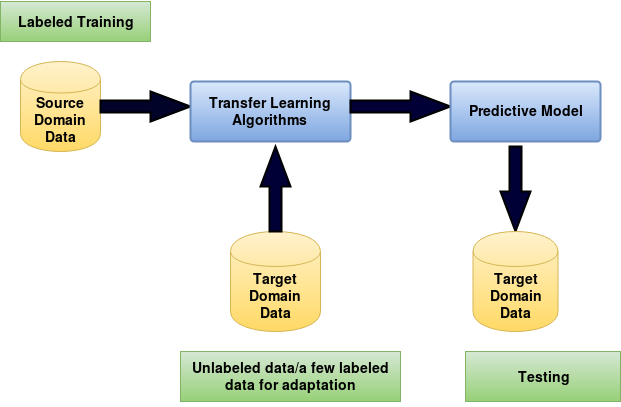
\includegraphics[width=1.1\linewidth]{Methodology.png}
	\caption{\textit{Diagram representing Flow diagram of methodology}}
	\label{Fig:1}
\end{figure}
%---------------------------------------------------------------------------


%\counterwithin{figure}{section}
\chapter*{}
\begin{figure}[!h]
  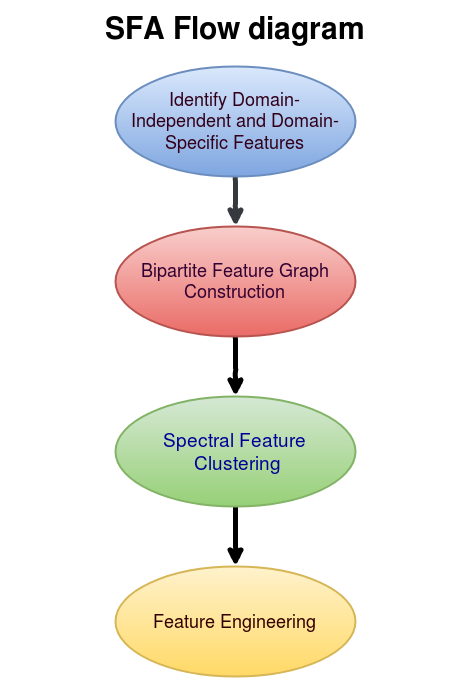
\includegraphics[width=0.9\linewidth]{SFA_flow_diagram.png}
  \caption{Figure representing flow of SFA Algorithm}
  \label{Fig:2}
\end{figure}




%----------------------------------------------------------------------------
\chapter{Methodology}

The main challenge of cross domain sentiment analysis (transfer learning) is to find  representation of cross domain sentiment data such that the gap between the source domain and target domain can be reduced.\\

We are using a Transfer Learning Algorithm called Spectral Feature Alignment (SFA) algorithm to find a new representation for cross-domain sentiment data, such that the gap between domains can be reduced. SFA uses some domain-independent words as a bridge to construct a bipartite graph to model the co-occurrence relationship between domain-specific words and domain-independent words.\\

This method involves following tasks -
\begin{enumerate}[label=\arabic*)]
\item To Recognize domain independent and domain specific features.
\item To align domain-specific features from different domains for cross-domain sentiment classification using spectral clustering method.
\item Train classifiers on the source using augmented features (original features + new features).
\end{enumerate}


\section{Recognising Domain-specific and Domain-independent Features}

Recognising Domain Independent and Domain Specific features is an important step in cross domain sentiment analysis. This is so because users express same sentiment using different words in different domains.
Consider a case of domain specific words  :-
Example - 'sharp' , 'compact' are used to express positive sentiment and 'blurry' for negative sentiment in case of Electronics while the same words carry no relevence in case of video games. In video games words like 'realistic' and 'hooked' are positive and 'boring' is negative.\\
\begin{itemize}
\item Due to domain specific words a classifier trained on one domain may not work on other domain.
\item Domain-independent features convey similar meaning in multiple domains or in the given source and target domains.\\
\end{itemize}

\subsection{Two methods to select domain-independent and domain-specific features :-} 
\begin{itemize}
\item \underline{\textbf{Method-1}} : A naive approach is to define a frequency threshold K1 and select domain-independent features based on the frequency of occurrence in both domains (i.e. features having frequency greater than K1 in both domains). Similarly, we define a frequency threshold K2 and select domain specific features based on its frequency of occurrence in a specific domain (i.e features having frequency greater than K2 in a specific domain).
\item \underline{\textbf{Method-2}} : In this method we adopt the idea of Diversity and Centrality which is reflected by Domain Independent and Domain Specific features respectively. Since we traverse both source and target domain to decide Domain Independent features therefore it signifies Diversity among both domains(can also be thought as global features). Similarly, Domain Specific features only requires traversal of a particular domain, therefore it signifies centrality of features in a domain.\\
For selecting domain independent features(i.e global features), we use frequency based threshold approach (as discussed in previous method).\\
For selecting domain specific features(i,e local features), we use mutual information based approach.\\
Mutual Information measures extent of dependence between features and domains.If a particular feature has high mutual information then it would be more dependent on a particular domain and therefore it is be more likely to be a domain specific feature.\\
To select set of domain specific features in specified domain, we will calculate mutual information of each feature with respect to a particular domain and take First T\% features with highest Mutual Information as Domain Specific features.\\

\end{itemize}

\begin{center}
\fbox{
\Large 
\( I(X^{i};D) = \sum\limits_{d \epsilon D} \sum\limits_{x\epsilon X^i ,x\neq 0} p(x,d)\log_2(\frac{p(x,d)}{p(x)p(d)}) \)
}
\end{center}


\begin{table}[!h]
\centering
\begin{tabular}{|p{2cm}|p{7cm}|p{7cm}|}
\hline
         & electronics                                                                                                                   & video games                                                                                         \\ \hline
positive & \textbf{Compact}; easy to operate; very \emph{good} picture quality; looks \textbf{sharp}!                                                             & "A very \emph{good} game! It is action packed and full of \emph{excitement}. I am very much \textbf{hooked} on this game." \\ \hline
positive & I purchased this unit from Circuit City and I was very \emph{excited} about the quality of the picture. It is really \emph{nice} and \textbf{sharp}. & Very \textbf{realistic} shooting action and \emph{good} plots. We played this and were \textbf{hooked}.                       \\ \hline
negative & It is also quite \textbf{blurry} in very dark settings. I will \emph{never} buy HP again.                                                     & The game is so \textbf{boring}. I am extremely unhappy and will probably \emph{never} buy Ubisoft again.            \\ \hline
\end{tabular}

\caption{Table representing Domain specific and Domain Independent Features}
\label{my-label}
\end{table}

\section{Bipartite Feature Graph Construction}

The co-occurrence relationship between domain-specific and domain-independent features is important for feature alignment across different domains. SFA uses domain-independent words as a bridge to construct a bipartite graph to model this co-occurrence relationship between domain-specific words and domain-independent words. The idea is that if two domain-specific words have connections to more common domain-independent words in the graph, they tend to be aligned together with higher probability. Similarly, if two domain-independent words have connections to more common domain-specific words in the graph, they tend to be aligned together with higher probability.\\
\linebreak
Based on the above method for selecting domain-independent and domain-specific features, we now construct a bipartite graph
\(G = (V_{DS} \cup V_{DI}, E)\) between them. In G, each vertex in \(V_{DS}\)
corresponds to a domain-specific word in \(W_{DS}\), and each vertex in
\(V_{DI}\) corresponds to a domain-independent word in \(W_{DI}\). An edge
in E connects two vertexes in \(V_{DS}\) and \(V_{DI}\) respectively.\\
\linebreak
Each edge \(e_{ij}\) \(\epsilon\) E is associated with a non-negative weight \(m_{ij}\). The score of \(m_{ij}\) measures the relationship between word \(w_i\) \(\epsilon\) \(W_{DS}\) and \(w_j\) \(\epsilon\) \(W_{DI}\) in \(D_{src}\) and \(D_{tar}\).
We have used the total number of co-occurrence of \(w_i\) \(\epsilon\) \(W_{DS}\) and \(w_j\) \(\epsilon\) \(W_{DI}\) in \(D_{src}\) and \(D_{tar}\). We can use other methods to estimate \(m_{ij}\), for example, we can use the distance between \(w_i\) and \(w_j\) to adjust the score of \(m_{ij}\).\\\linebreak
A bipartite graph example is shown in Figure 5.1, which is constructed based on the example shown in Table 5.1.\\
\begin{table}[!h]
\begin{center}
\label{my-label}
\begin{tabular}{|p{2cm}|p{2cm}|p{2cm}|p{2cm}|p{2cm}|p{2cm}|p{2cm}|}
\hline
                    & \large\textbf{compact} & \large\textbf{realistic} & \large\textbf{sharp} & \large\textbf{hooked} & \large\textbf{blurry} & \large\textbf{boring} \\ \hline
\large\textbf{good}       \large & 1               \large & 1                 \large & 1             \large & 1               & 0               & 0               \\ \hline
\large\textbf{exciting}   & 0                & 0                  & 1              & 1               & 0               & 0               \\ \hline
\large\textbf{never\_buy} & 0                & 0                  & 0              & 0               & 1               & 1               \\ \hline
\end{tabular}
\end{center}
\caption{\textit{A co-occurrence matrix of domain-specific and domain-independent words}}

\end{table}

\begin{figure}[!h]
	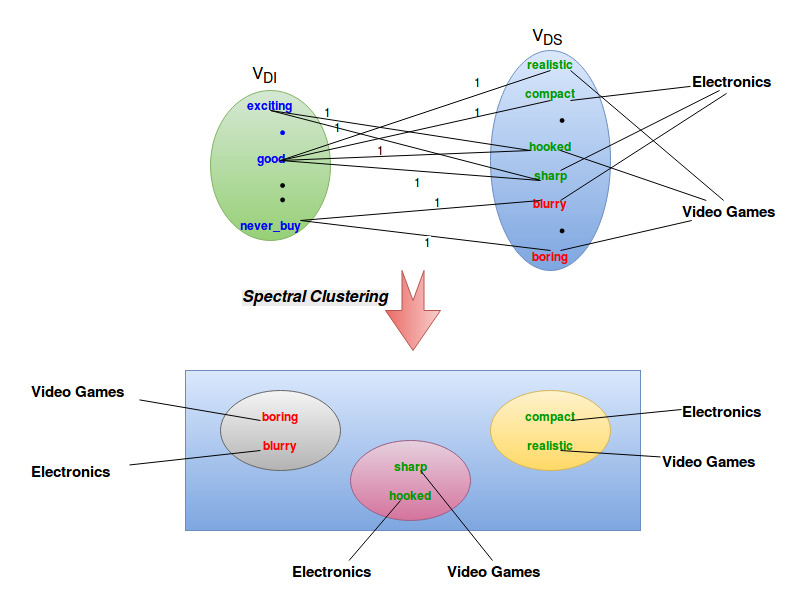
\includegraphics[width=\linewidth]{SpectralClustering.jpg}
	\caption{\textit{Bipartite graph and Spectral Clustering\cite{Pan:2010:CSC:1772690.1772767}}}
	\label{Fig:2}
\end{figure}

Now we can use the constructed bipartite graph to model the intrinsic relationship between domain-specific and domain-independent features.\\

\subsection{Implementation :}
\textbf{Some Terms :-}\\
co-occurence \quad - \quad co-occurence matrix.\\
\(wt(w_{i},w_{j})\) \quad - \quad edge weight between \(w_{i}\) and \(w_{j}\).\\
\(w_{specific}\) \quad - \quad a specific word.\\
\(w_{independent}\) \quad - \quad an independent word.\\
\(S_{article}\) \quad - \quad set of all articles in source corpus.\\
\(T_{article}\) \quad - \quad set of all artcles  in target corpus. \\
\linebreak
We represent the bipartite graph as a co-occurence matrix. In our method we have given edge weight \(wt\) to co-occurence\([w_{specific}][w_{independent}]\) and co-occurence\([w_{independent}][w_{specific}]\) if \(w_{specific}\) and \(w_{independent}\) occur together in an article.\\
\linebreak
\textbf{Weighting techniques :-}
\\
We have used two weighing techniques to construct the bipartite graph of specific and independent features.
\begin{enumerate}
\item \textbf{Frequency based weighting} : The first method counts the total number of times \(w_{specific}\) occurs with \(w_{independent}\) in a article for each article of set \(S_{article}\) and \(T_{article}\) .
\begin{center}
\fbox{
\Large 
\(wt(w_{specific}, w_{independent})= \sum\limits_{l1}^{} \sum\limits_{l2}^{} \)(count of \(w_{specific}\) with \(w_{independent}\) in article A)
}
\\
\end{center}
l1 = A element of \((S_{article}\bigcup T_{article})\)\\ 
l2 = \(w_{specific}\) and \(w_{independent}\) element of article A

\item \textbf{Distance based weighting} : In this method we make use of distance between \(w_{specific}\) and \(w_{independent}\) in a article. The value added for each occurence of \(w_{specific}\) with \(w_{independent}\) and vice versa decreases with increase in distance between them.
\begin{center}
\fbox{
\Large 
\(wt(w_{specific}, w_{independent})\) = \(\sum\limits_{L1}^{} \sum\limits_{L2}^{}\)(1000\(\times\)(\(\frac{1}{(1 + abs(posI(w_{independent}) - posS(w_{specific})))}\) ))
}
\\
\end{center}
L1 = A element of (\(S_{article}\) \(\bigcup\) \(T_{article}\))\\
L2 = \(w_{specific}\) and \(w_{independen}\) element of article A.\\
posI gives position of \(w_{independent}\) , in article A ignoring specific words.\\
posS gives position of \(w_{specific}\) , in article A ignoring independent words.\\
\end{enumerate}

\section{Spectral Feature Clustering}

Now, to align domain-specific features so as to reduce the gap between domains, we will need to do some type of clustering on the domain-specific and domain-independent features.\\
\linebreak
For doing this, we will now adapt a spectral clustering algorithm on the feature bipartite graph we made before.\\
\linebreak
In graph spectral theory, one of the main assumptions is:\\
\emph{if two nodes in a graph are connected to many common nodes,
then they should be very similar (or quite related)}.\\
\linebreak
\subsection{Spectral Clustering:}
Spectral clustering technique make use of the spectrum (eigenvalues) of the similarity matrix of the data to perform dimensionality reduction before clustering in fewer dimensions.\\
The similarity matrix is provided as an input and consists of a quantitative assessment of the relative similarity of each pair of points in the dataset.\\
\linebreak
It is mainly divided into two parts: 
\begin{enumerate}[label=\arabic*.]
\item Feature Reduction
\item Any traditional clustering algorithm like k-means clustering.
\end{enumerate}

Firstly we\(\textquotesingle \)ll discuss the Feature Reduction part:
\begin{enumerate}[label=\alph*).]
\item The input is Affinity/Similarity matrix (A):
\[A_{ij}  =    \begin{cases} 
      w_{ij} & :weight \ of \ edge(i,j) \\
      0 & :no \  edge 
   \end{cases}
\]
\item Then we calculate Laplacian Matrix (L) of matrix A:
\[ L = D^{-1/2} A D^{-1/2} \]
\quad \quad where \(D_{ii}\) = \(\sum\limits_{j}^{} A_{ij}\)\\
\item Calcualtion of Eigen value \& Eigen vectors
Sorting eigen valuesion decreasing order\\
\(\lambda \textsubscript{1} \ , \ \lambda \textsubscript{2} \ , \ \lambda \textsubscript{3} \ , \ . \ . \ . \ . \ . \  \ , \ \lambda \textsubscript{n}\) \ are \ eigen \ values \ .\\
\(\mu \textsubscript{1} \ , \ \mu \textsubscript{2} \ , \ \mu \textsubscript{3} \ , \ . \ . \ . \ . \ . \  \ , \ \mu \textsubscript{n}\) \ are \ eigen \ vectors \ .\\
\linebreak
Spectrum of Graph : Set of eigen vectors of laplacian matrix
\( \lambda \textsubscript{2} \ - \) defines algebraic connectivity of graph i.e. more the value of \( \lambda \textsubscript{2}\), more density of connected graph.\\
\item Partioning of the Graph:
\begin{enumerate}[label=\roman*).]
\item Selection of first K-eigen vectors according to sorted list of eigen values.
\item We define \(U \  \epsilon  \  \mathbb{R}^{m\times k}\) 
\item Normalization \(U_{ij} = \frac{U_{ij}}{(\sum\limits_{j}^{} U_{ij}^2 )^{1/2}}\)
\item Apply k-means clustering on U.\\
\end{enumerate}
So, after doing all the four steps we reduced our feature set from \(m\times m\) size to \(m\times k\) features.\\
Once the feature set is reduced, then we go for clustering algorithm.\\
\end{enumerate}
Second part : Clustering
\begin{enumerate}[label=\alph*).]
\item It is done by applying the k-means clustering on the new reduced feature set obtained by spectral reduction.
\item This k-means algorithm clusterd the n-point into k clusters. 
\end{enumerate}
In our case, we assume:\\
\begin{enumerate}[label=\arabic*.]
\item if two domain-specific features are connected to many common domain- independent features, then they tend to be very related and will be aligned to a same cluster with high probability,
\item if two domain-independent features are connected to many common domain-specific features, then they tend to be very related and will be aligned to a same cluster with high probability.
\end{enumerate}
Finally, Using the above assumptions and the weighted feature bipartite graph, we align the domain-specific features of both the domains into k clusters, where k is an input parameter.

\section{Feature Engineering}

After applying Spectral Clustring algorithm on the bipartite graph of features we have a set of clusters. Each cluster contains some domain specific and some domain independent words.As already discussed, domain specific words which convey similar sentiment will be placed in same cluster with high probability. We can use this property of clusters to modify our corpus in a manner that will make it easier for us to tranfer knowledge.
Since,  domain independent knowledge can be transfered without any extra effort we have to focus on domain specific words.

In our method, we will replace each domain specific word occuring in \(i^{th}\) cluster with cluster\_i, (since this type of word is less likely to appear in an article) let\textquotesingle s call this as cluster name of a domain specific word. Next step is to replace all the occurences of a word \(w_{specific}\) in Source corpus and Target corpus with its corresponding cluster name. This way, we reduced the gap between domain specific words of the two domains, which is the primary objective of this algorithm. Now, each corpus contains domain independent words and cluster words (specific words replaced with their cluster names).

Using the modified Source corpus we can train our model to predict sentiments of articles in the target domain.\\

%------------------------------------------------------------------------------

\chapter{Proposed Models}

Using above algorithm we have created three models for cross-domain sentiment analysis.\\
The models vary mainly in two steps :-
\begin{enumerate}
\item Finding domain independent and domain specific features.
\item Weighting scheme of bi-partite graph.
\end{enumerate}

\section{Model-1 :}
\begin{enumerate}
\item Finding domain independent and domain specific features :-\\
used frequency based approach to segregate independent and specific features.
\item Calculating edges of bipartite graph :-\\
used frequency based weighing technique to calulate edges of bipartite graph.
\end{enumerate}
\section{Model-2 :}
\begin{enumerate}
\item Finding domain independent and domain specific features :-\\
used mutual information of features with domain as parameter to select domain independent and specific features.
\item Calculating edges of bipartite graph :-\\
same as Model-1.
\end{enumerate}
\section{Model-3 :}
\begin{enumerate}
\item Finding domain independent and specific features :-\\
same as Model-2.
\item Calculating edges of bipartite graph :-\\
used distance based weighting.
\end{enumerate}

%----------------------------------------------------------------------------------------

%\begin{multicols}{2}
\chapter{Dataset Description}
Our model needs set of correlated datasets for better demonstration of cross domain sentiment analysis.
Therefore, we picked collection of product reviews from Amazon.\\
\linebreak
The reviews are about four product domains:\\
Books(B), Dvds(D), Electronics(E) and Kitchen Appliances(K).\\
\linebreak
Each review is assigned a sentiment label, $-$1 (negative review) or $+$1 (positive review), based on the
review of the products. Each domain has around 800 positive reviews and negative reviews.
Using these datasets, we can create 12 pairs of source and target domains for cross-domain sentiment classification, namely:\\
\linebreak
D\(\rightarrow\)B, E\(\rightarrow\)B,  K\(\rightarrow\)B,  K\(\rightarrow\)E,  D\(\rightarrow\)E,  B\(\rightarrow\)E,  B\(\rightarrow\)D,  K\(\rightarrow\)D,  E\(\rightarrow\)D,  B\(\rightarrow\)K,  D\(\rightarrow\)K,  E\(\rightarrow\)K,\\
\linebreak 
where the word before an arrow corresponds with the source domain and the word after an arrow corresponds with the target domain.\\

%------------------------------------------------------------------------------

\chapter{Experiments}

\section{Model-1 :}
The different hyperparameters used in our Model-1:
\begin{enumerate}[label=\alph*.)]
\item Domain Independent feature frequency cutoff, [IFC] The words which are present in both source and target datasets with frequency greater than this value are only considered as Independent features.\\
Range:- [10, 15, 20, 25, 30].
\item Domain Specific feature frequency cutoff, [SFC] The words which are present in one or both of the datasets with a frequnency less than this value are only considered as specific features.\\
Range:- [10, 15, 20, 25, 30].
\item No. of clusters assumed for clustering. [NCC]\\
Range:- [10, 20, 30, 40, 50].
\end{enumerate}
So for each of the above combination of datasets we tried all \((5\times 5\times 5)\) 125
combinations.
\section{Model-2 :}
The way we did variations for different hyperparameters in our Model-2 is as follows:
\begin{enumerate}[label=\alph*.)]
\item Domain Independent feature frequency cutoff, [IFC] The words which are present in both source and target datasets with frequency greater than this value are only considered as Independent features.\\
Range:- [10, 15, 20, 25, 30].
\item Mutual information of features with a domain is calculated. The result is stored in two seperate lists , source features list and target features list. The lists are sorted in descending order of mutual information. Top features from each list are selected as specific features belonging to corresponding domain.\\
Range:- top x percent features are selected x element [33,12.5,7.7,5.6,4.35]
\item No. of clusters assumed for clustering. [NCC]\\
Range:- [10, 20, 30, 40, 50].
\end{enumerate}
So for each of the above combination of datasets we tried all \((5\times 5\times 5)\) 125
combinations.
\section{Model-3 :}
In method 3 all hyperparameters are same as that of Model-2. In Model-3 the we have used a distance based weighting approach to calculate edge weights of bipartite graph.

% Please add the following required packages to your document preamble:
% \usepackage{longtable}
% Note: It may be necessary to compile the document several times to get a multi-page table to line up properly
\begin{longtable}[c]{|l|l|l|l|l|l|}
\hline
Source \ \ & Target & No. of Clusters & \begin{tabular}[c]{@{}l@{}}Specific    \\ Cutoff\end{tabular} & \begin{tabular}[c]{@{}l@{}}Independent \\ Cutoff\end{tabular} & Accuracy \\ \hline
\endfirsthead
%
\endhead
%
electronics & \begin{tabular}[c]{@{}l@{}}kitchen \&\\ housewares\end{tabular} & 20 & 10 & 10 & 80.75 \\ \hline
\begin{tabular}[c]{@{}l@{}}kitchen \&\\ housewares\end{tabular} & electronics & 10 & 30 & 20 & 79.4 \\ \hline
books & dvd & 30 & 10 & 25 & 78.7 \\ \hline
dvd & books & 30 & 15 & 25 & 77.85 \\ \hline
dvd & \begin{tabular}[c]{@{}l@{}}kitchen \&\\ housewares\end{tabular} & 20 & 10 & 10 & 71.8 \\ \hline
\begin{tabular}[c]{@{}l@{}}kitchen \&\\ housewares\end{tabular} & dvd & 50 & 20 & 10 & 71.5 \\ \hline
electronics & dvd & 40 & 30 & 25 & 70.7 \\ \hline
dvd & electronics & 40 & 10 & 10 & 68.7 \\ \hline
electronics & books & 50 & 30 & 25 & 68.1 \\ \hline
books & \begin{tabular}[c]{@{}l@{}}kitchen \&\\ housewares\end{tabular} & 30 & 25 & 15 & 67.75 \\ \hline
\begin{tabular}[c]{@{}l@{}}kitchen \&\\ housewares\end{tabular} & books & 40 & 25 & 15 & 67.15 \\ \hline
books & electronics & 30 & 10 & 25 & 66.8 \\ \hline
\caption{\footnotesize Table for Model-1 consisting of Ideal hyperparameters after parameter tuning and corresponding Accuracy for each combinations of different datasets}
\label{my-label}\\
\end{longtable}

%---------------------

% Please add the following required packages to your document preamble:
% \usepackage{longtable}
% Note: It may be necessary to compile the document several times to get a multi-page table to line up properly
\begin{longtable}[c]{|l|l|l|l|l|l|}
\hline
Source\ \ & Target & No. of Clusters & \begin{tabular}[c]{@{}l@{}}Specific\\ Cutoff\end{tabular} & \begin{tabular}[c]{@{}l@{}}Independent\\ Cutoff\end{tabular} & Accuracy \\ \hline
\endfirsthead
%
\endhead
%
electronics & \begin{tabular}[c]{@{}l@{}}kitchen \& \\ housewares\end{tabular} & 20 & 3 & 15 & 80.65 \\ \hline
\begin{tabular}[c]{@{}l@{}}kitchen \&\\ housewares\end{tabular} & electronics & 15 & 3 & 10 & 79.5 \\ \hline
books & dvd & 15 & 3 & 20 & 78.7 \\ \hline
dvd & books & 35 & 8 & 30 & 78.2 \\ \hline
dvd & \begin{tabular}[c]{@{}l@{}}kitchen \&\\ housewares\end{tabular} & 30 & 13 & 10 & 72 \\ \hline
\begin{tabular}[c]{@{}l@{}}kitchen \&\\ housewares\end{tabular} & dvd & 35 & 23 & 10 & 71.4 \\ \hline
electronics & dvd & 25 & 3 & 15 & 71.3 \\ \hline
dvd & electronics & 30 & 3 & 15 & 69.1 \\ \hline
electronics & books & 30 & 8 & 10 & 68.3 \\ \hline
books & electronics & 30 & 3 & 20 & 67.9 \\ \hline
books & \begin{tabular}[c]{@{}l@{}}kitchen \&\\ housewares\end{tabular} & 25 & 13 & 10 & 67.7 \\ \hline
\begin{tabular}[c]{@{}l@{}}kitchen \&\\ housewares\end{tabular} & books & 15 & 3 & 10 & 67.4 \\ \hline
\caption{Table for Model-2 consisting of Ideal hyperparameters after parameter tuning and corresponding Accuracy for each combinations of different datasets}
\label{my-label}\\
\end{longtable}

%---------------------

% Please add the following required packages to your document preamble:
% \usepackage{longtable}
% Note: It may be necessary to compile the document several times to get a multi-page table to line up properly
\begin{longtable}[c]{|l|l|l|l|l|l|}
\hline
Source \ \                                                          & Target                                                          & No. of Clusters & \begin{tabular}[c]{@{}l@{}}Specific\\ Cutoff\end{tabular} & \begin{tabular}[c]{@{}l@{}}Independent\\ Cutoff\end{tabular} & Accuracy \\ \hline
\endfirsthead
%
\endhead
%
electronics                                                     & \begin{tabular}[c]{@{}l@{}}kitchen \&\\ housewares\end{tabular} & 30              & 8                                                         & 10                                                           & 80.55    \\ \hline
\begin{tabular}[c]{@{}l@{}}kitchen \&\\ housewares\end{tabular} & electronics                                                     & 35              & 3                                                         & 20                                                           & 79.55    \\ \hline
books                                                           & dvd                                                             & 20              & 23                                                        & 25                                                           & 78.9     \\ \hline
dvd                                                             & books                                                           & 35              & 3                                                         & 30                                                           & 77.95    \\ \hline
dvd                                                             & \begin{tabular}[c]{@{}l@{}}kitchen \&\\ housewares\end{tabular} & 25              & 3                                                         & 10                                                           & 72.45    \\ \hline
\begin{tabular}[c]{@{}l@{}}kitchen \&\\ housewares\end{tabular} & dvd                                                             & 35              & 23                                                        & 10                                                           & 71.25    \\ \hline
electronics                                                     & dvd                                                             & 10              & 3                                                         & 25                                                           & 70.85    \\ \hline
dvd                                                             & electronics                                                     & 30              & 8                                                         & 30                                                           & 69.15    \\ \hline
books                                                           & \begin{tabular}[c]{@{}l@{}}kitchen \&\\ housewares\end{tabular} & 20              & 8                                                         & 10                                                           & 69.1     \\ \hline
electronics                                                     & books                                                           & 30              & 8                                                         & 25                                                           & 68.75    \\ \hline
\begin{tabular}[c]{@{}l@{}}kitchen \&\\ housewares\end{tabular} & books                                                           & 30              & 23                                                        & 15                                                           & 68.05    \\ \hline
books                                                           & electronics                                                     & 30              & 3                                                         & 20                                                           & 67.6     \\ \hline
\caption{Table for Model-3 consisting of Ideal hyperparameters after parameter tuning and corresponding Accuracy for each combinations of different datasets}
\label{my-label}\\
\end{longtable}

%-----------------------

% Please add the following required packages to your document preamble:
% \usepackage{longtable}
% Note: It may be necessary to compile the document several times to get a multi-page table to line up properly
\begin{longtable}[c]{|l|l|l|l|l|}
\hline
Source \ \ & Target \ \ & Method 1 & Method 2 & Method 3 \\ \hline
\endfirsthead
%
\endhead
%
electronics & \begin{tabular}[c]{@{}l@{}}kitchen \&\\ housewares\end{tabular} & 80.75 & 80.65 & 80.55 \\ \hline
\begin{tabular}[c]{@{}l@{}}kitchen \&\\ housewares\end{tabular} & electronics & 79.4 & 79.5 & 79.55 \\ \hline
books & dvd & 78.7 & 78.7 & 78.9 \\ \hline
dvd & books & 77.85 & 78.2 & 77.95 \\ \hline
dvd & \begin{tabular}[c]{@{}l@{}}kitchen \&\\ housewares\end{tabular} & 71.8 & 72 & 72.45 \\ \hline
\begin{tabular}[c]{@{}l@{}}kitchen \&\\ housewares\end{tabular} & dvd & 71.5 & 71.4 & 71.25 \\ \hline
electronics & dvd & 70.7 & 71.3 & 70.85 \\ \hline
dvd & electronics & 68.7 & 69.1 & 69.15 \\ \hline
books & \begin{tabular}[c]{@{}l@{}}kitchen \&\\ housewares\end{tabular} & 68.1 & 68.3 & 69.1 \\ \hline
electronics & books & 67.75 & 67.9 & 68.75 \\ \hline
\begin{tabular}[c]{@{}l@{}}kitchen \&\\ housewares\end{tabular} & books & 67.15 & 67.7 & 68.05 \\ \hline
books & electronics & 66.8 & 67.4 & 67.6 \\ \hline
\caption{Comparison of Accuracy obtained by using different models proposed in the report on different combinations of datasets}
\label{my-label}\\
\end{longtable}


%-----------------------------------------------------------------------

\chapter{Graphs}
For each method we implemented, there are three graphs which shows how the accuracy (best) changes with respect to variation of the 3 hyperparameters, namely
\begin{enumerate}[label=\arabic*]
\item Accuracy vs. No. of clusters.
\item Accuracy vs. Specific threshold value.
\item Accuracy vs. Independent threshold value.
\end{enumerate}
Each graph shows the accuracy for all the datasets, (datasets represented by different colors).
\\
Finally we plotted a graph which shows how accuracy for a specific pair of dataset changes with respect to different methods.

\section{Model-1 :}

\myfigure{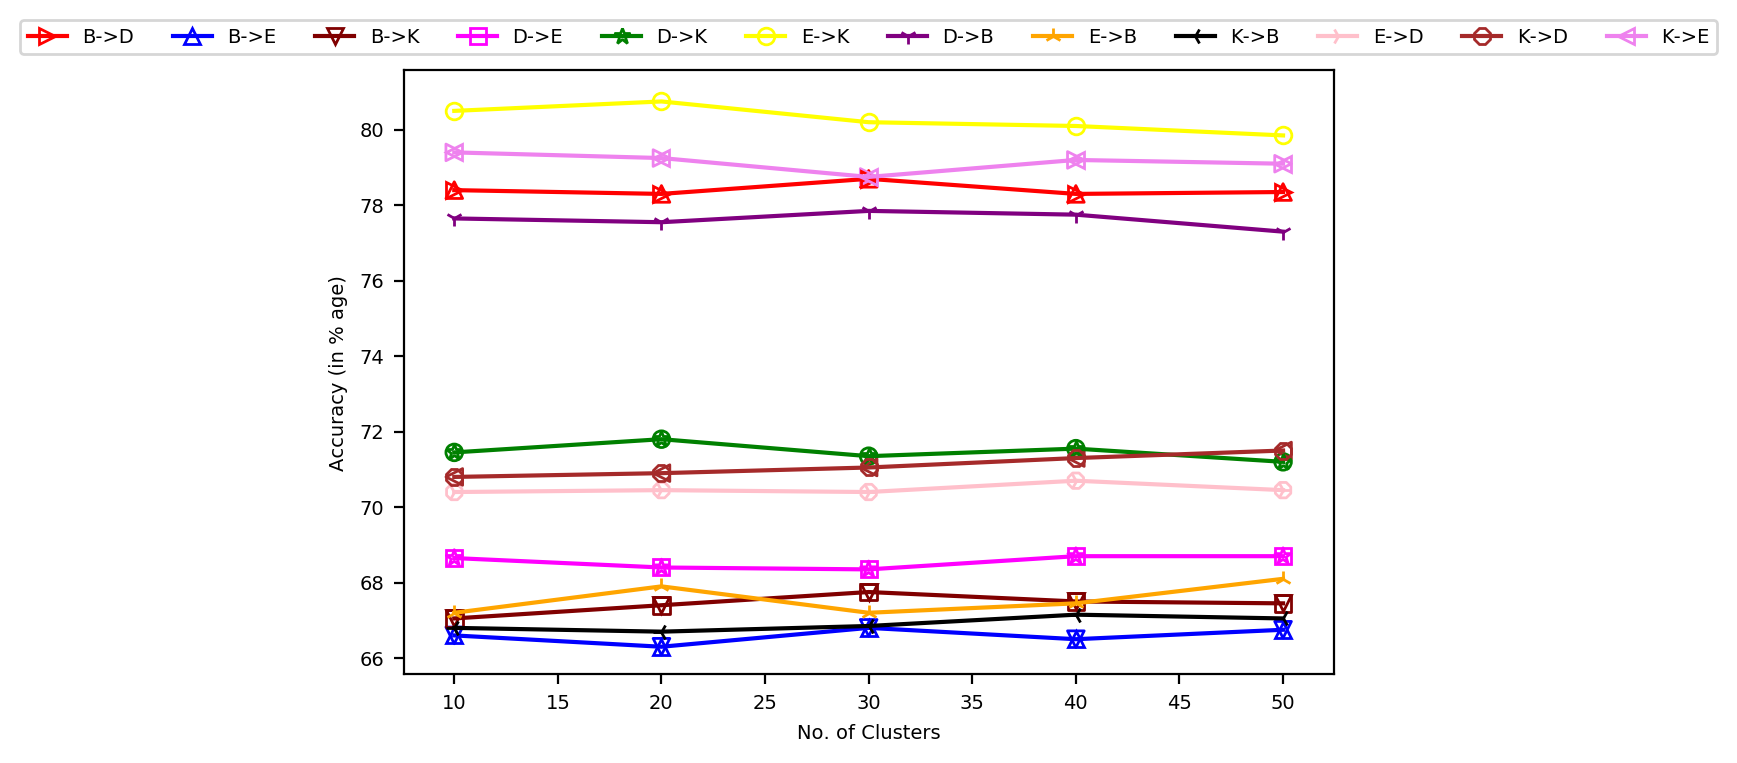
\includegraphics[width=1.1\textwidth]{m1c.png}
\figcaption{\emph { Accuracy(best) vs Number of Clusters}}}

\myfigure{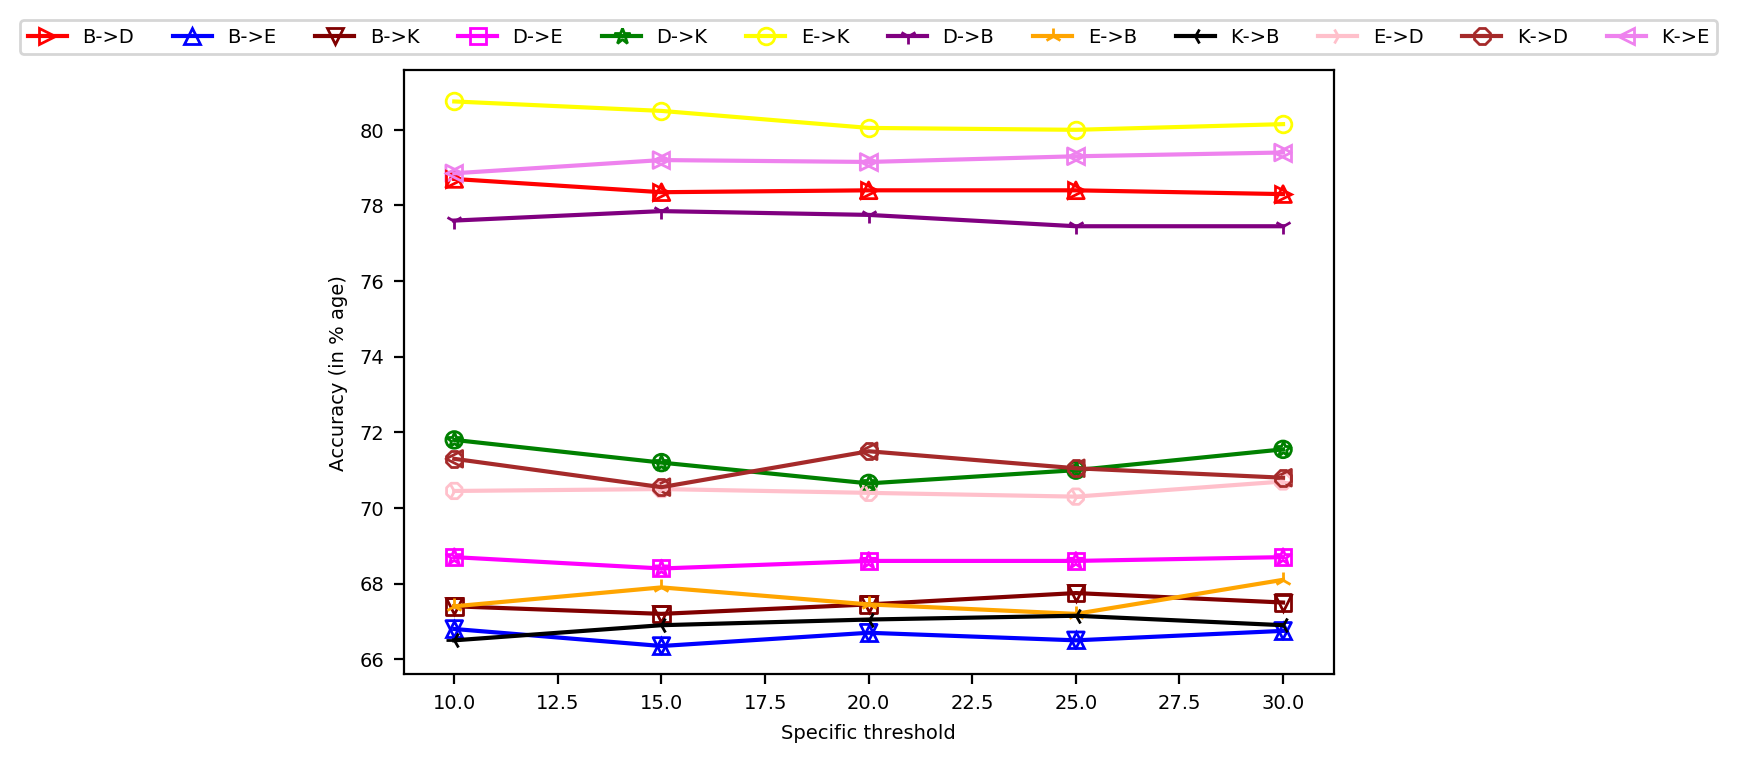
\includegraphics[width=1.1\textwidth]{m1s.png}
\figcaption{\emph { Accuracy(best) vs Specific Threshold}}}

\myfigure{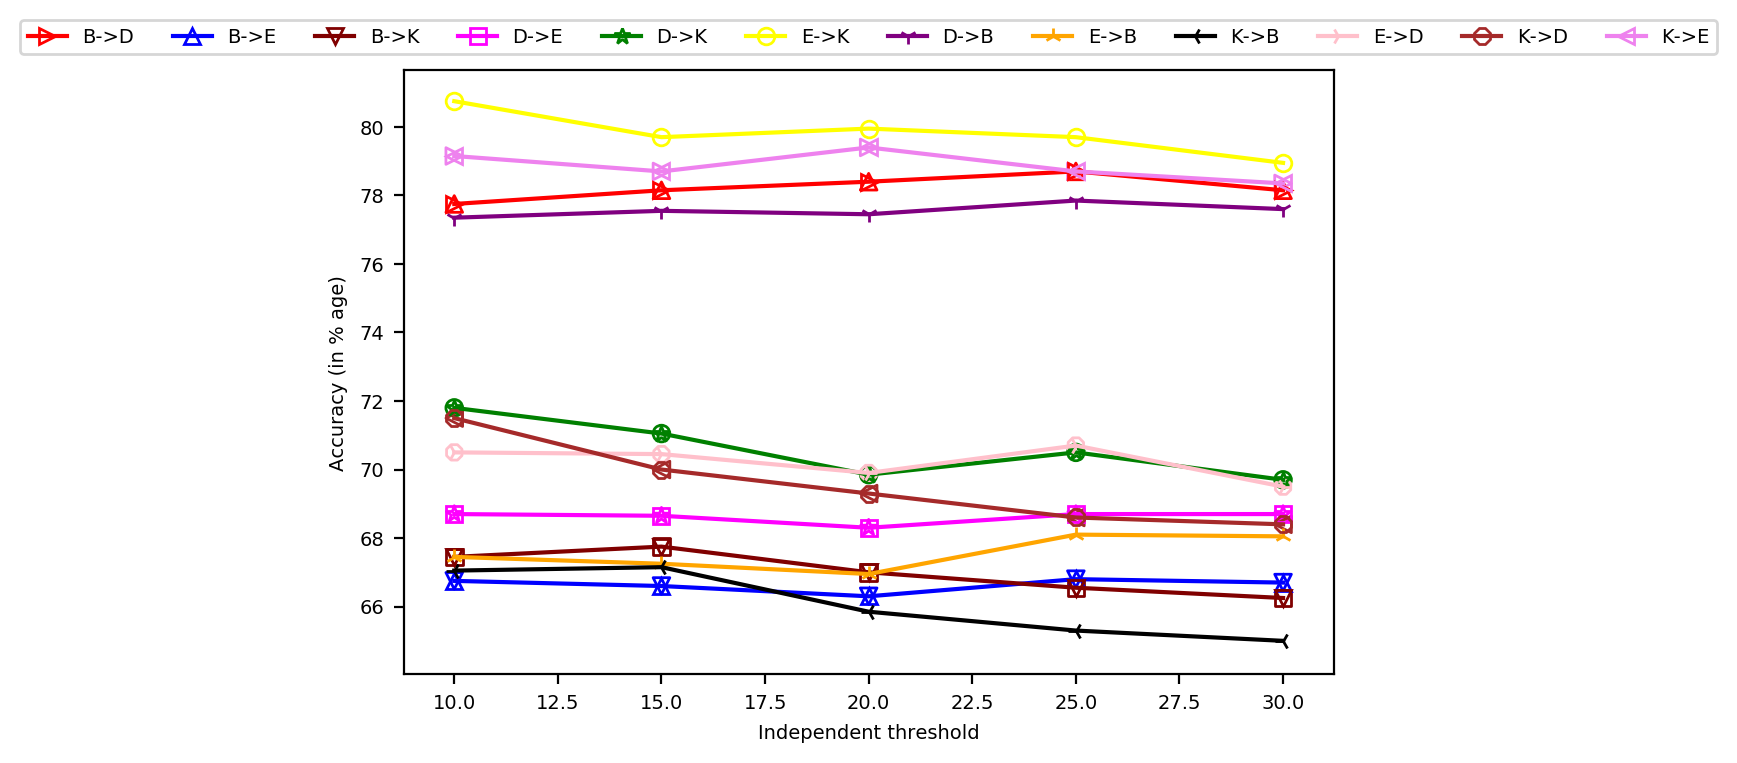
\includegraphics[width=1.1\textwidth]{m1i.png}
\figcaption{\emph { Accuracy(best) vs Independent Threshold}}}

\section{Model-2 :}

\myfigure{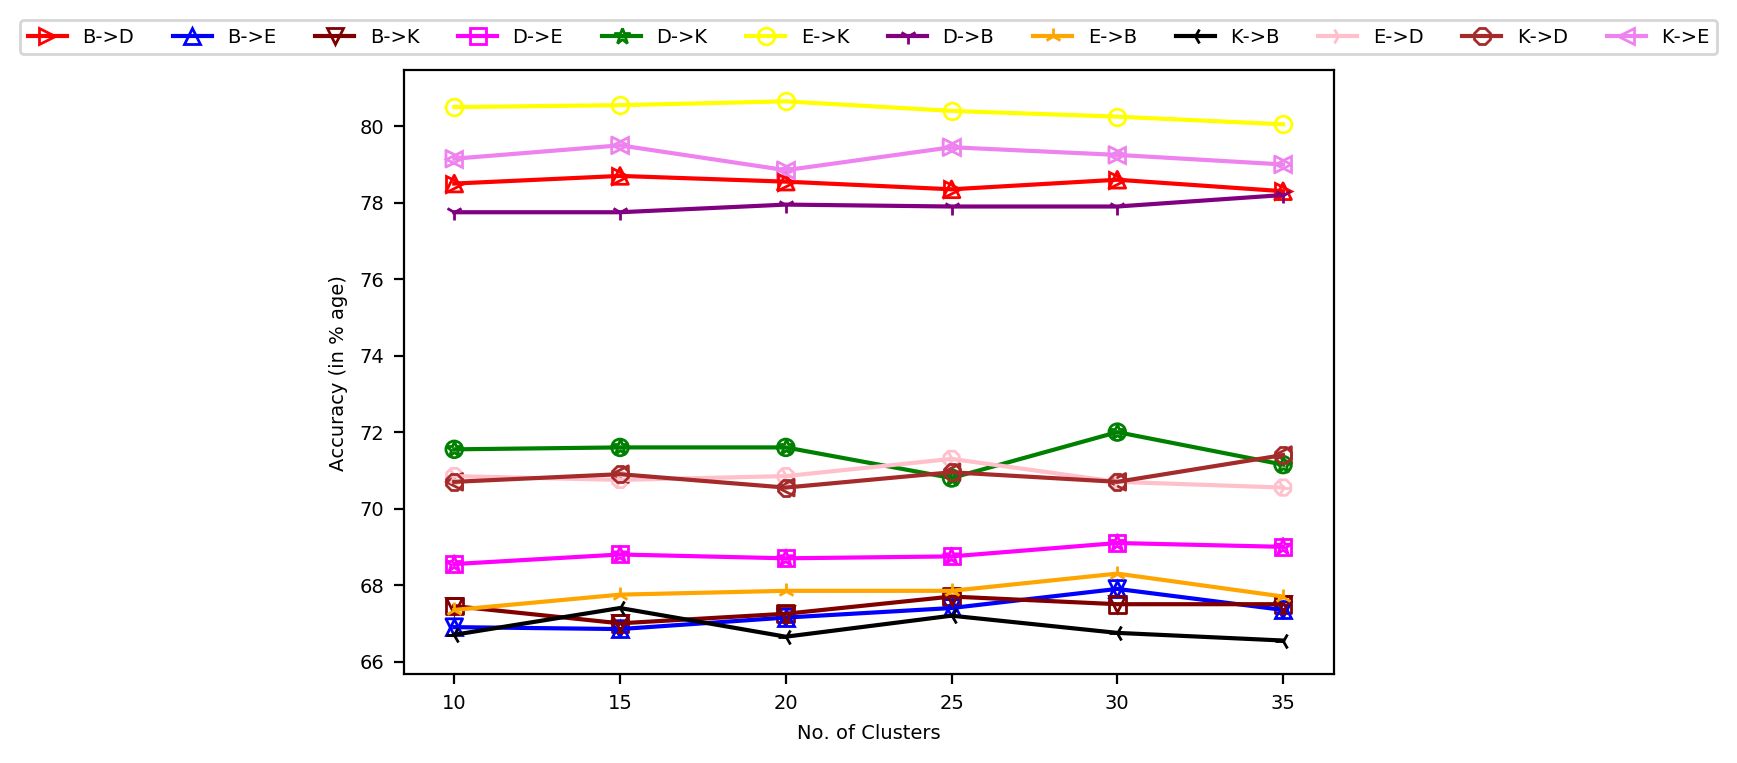
\includegraphics[width=1.1\textwidth]{m2c.png}
\figcaption{\emph { Accuracy(best) vs Number of Clusters}}}

\myfigure{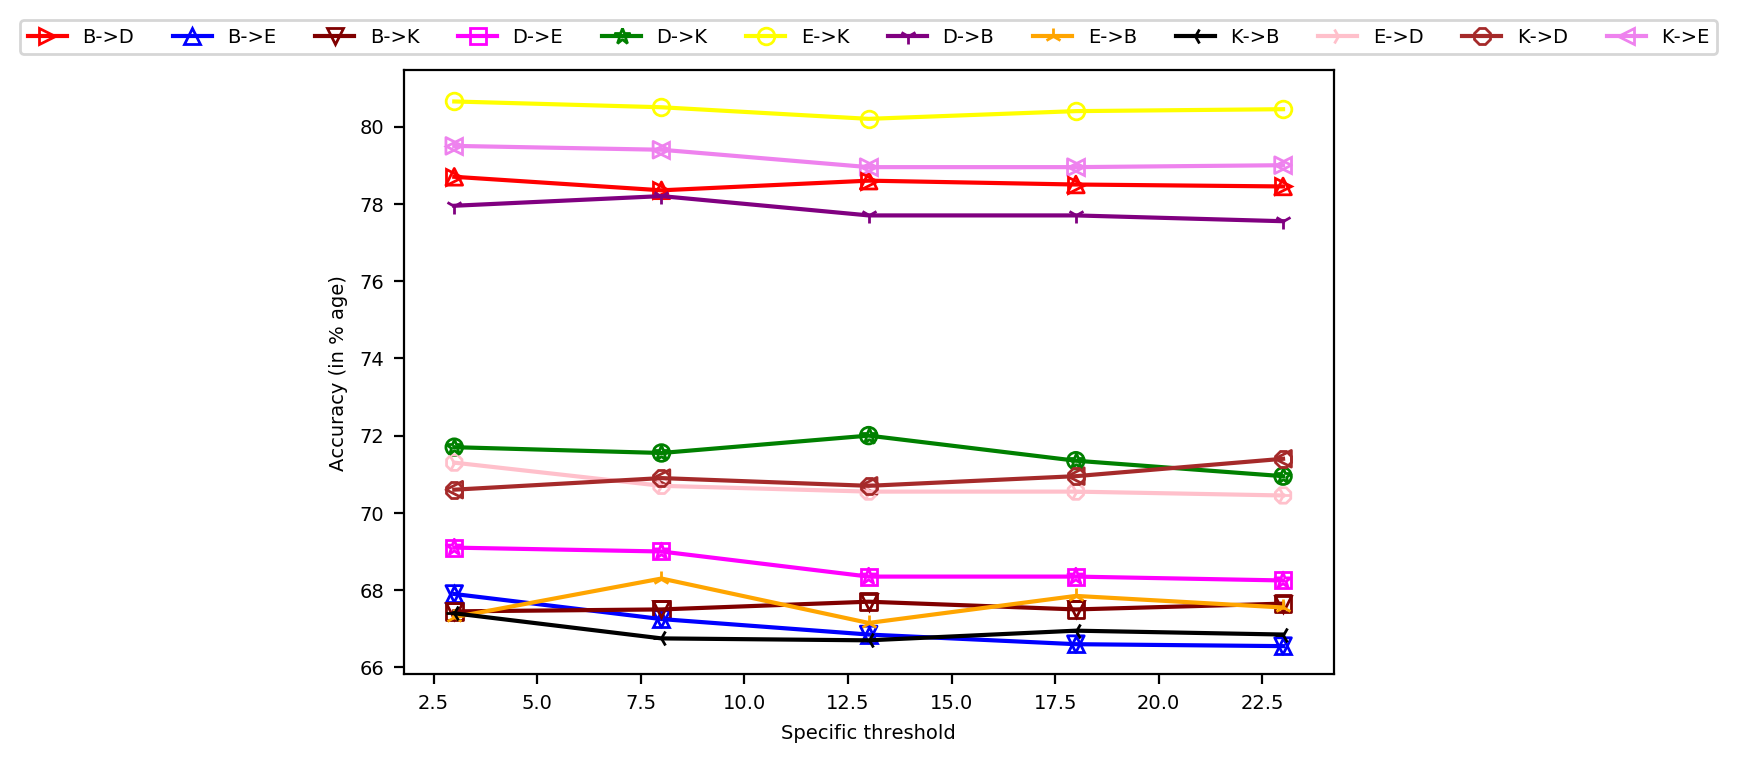
\includegraphics[width=1.1\textwidth]{m2s.png}
\figcaption{\emph { Accuracy(best) vs Specific Threshold}}}

\myfigure{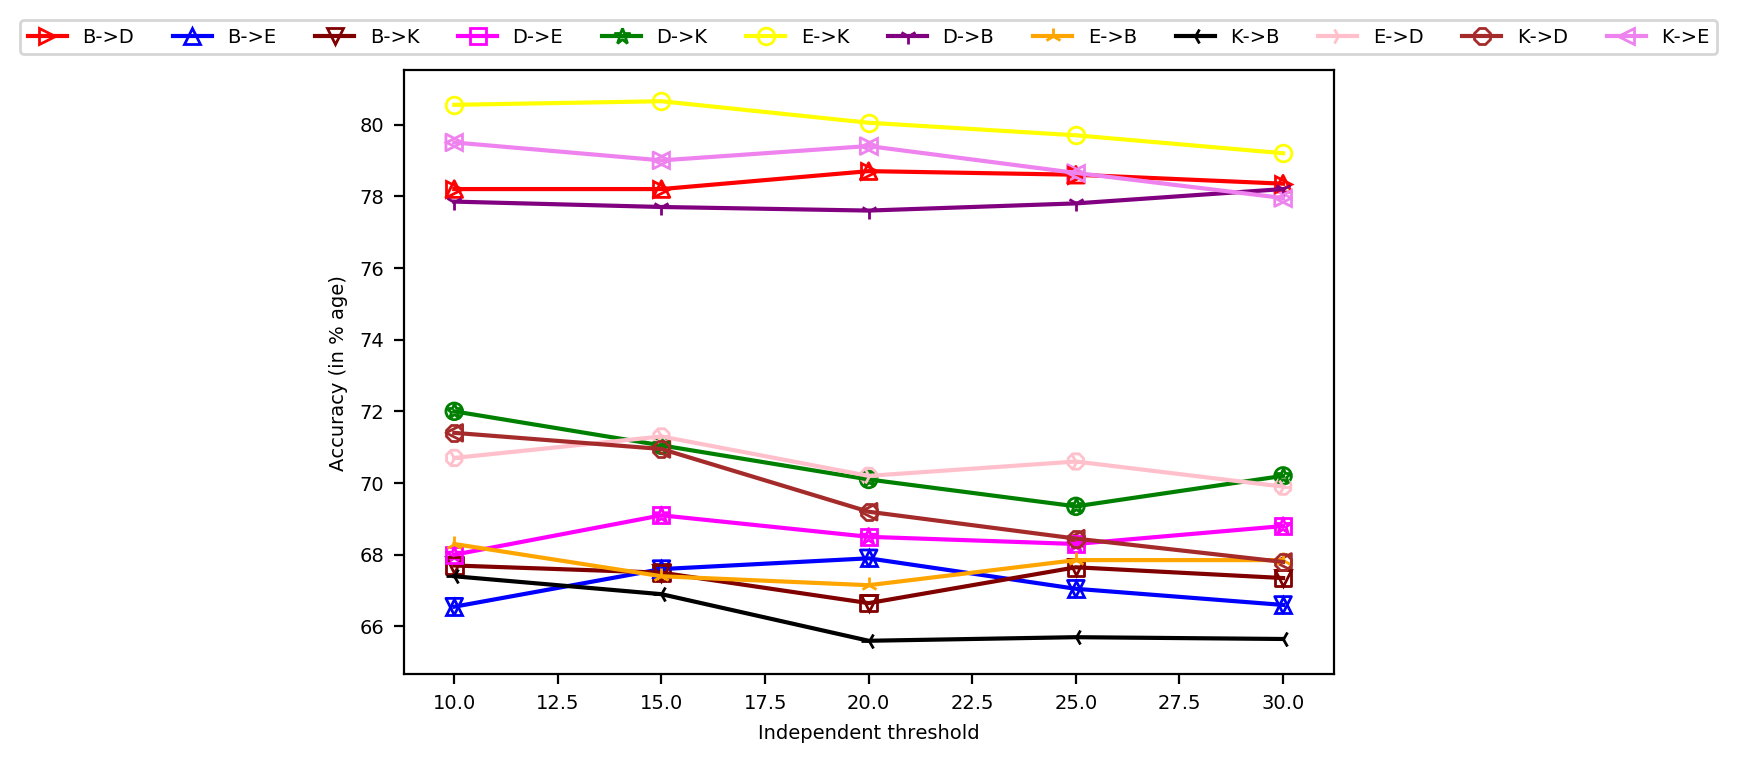
\includegraphics[width=1.1\textwidth]{m2i.png}
\figcaption{\emph { Accuracy(best) vs Independent Threshold}}}

\section{Model-3 :}

\myfigure{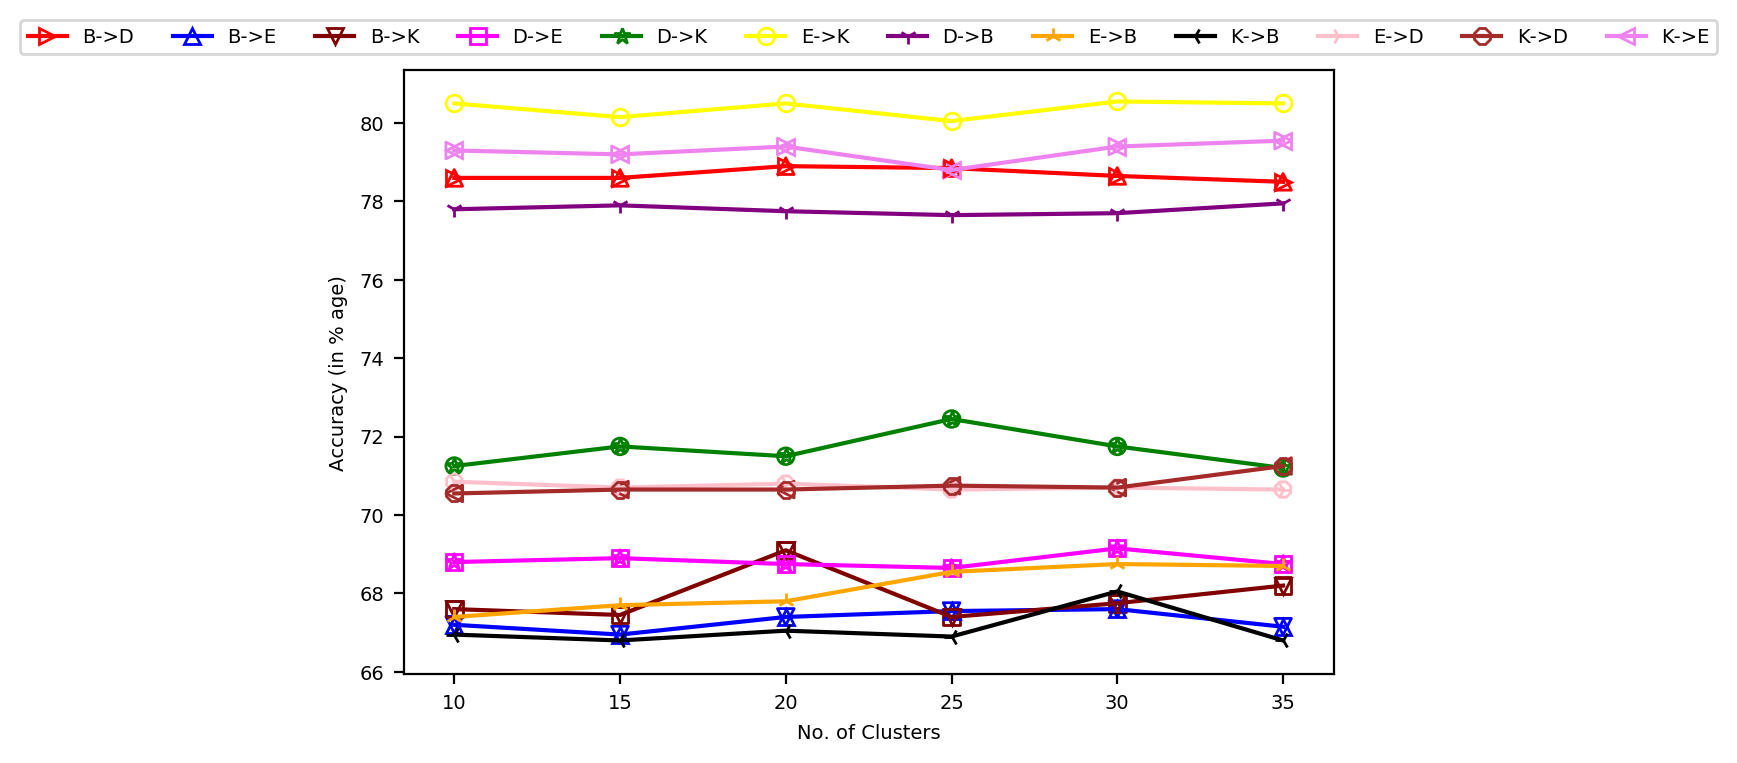
\includegraphics[width=1.1\textwidth]{m3c.png}
\figcaption{\emph { Accuracy(best) vs Number of Clusters}}}

\myfigure{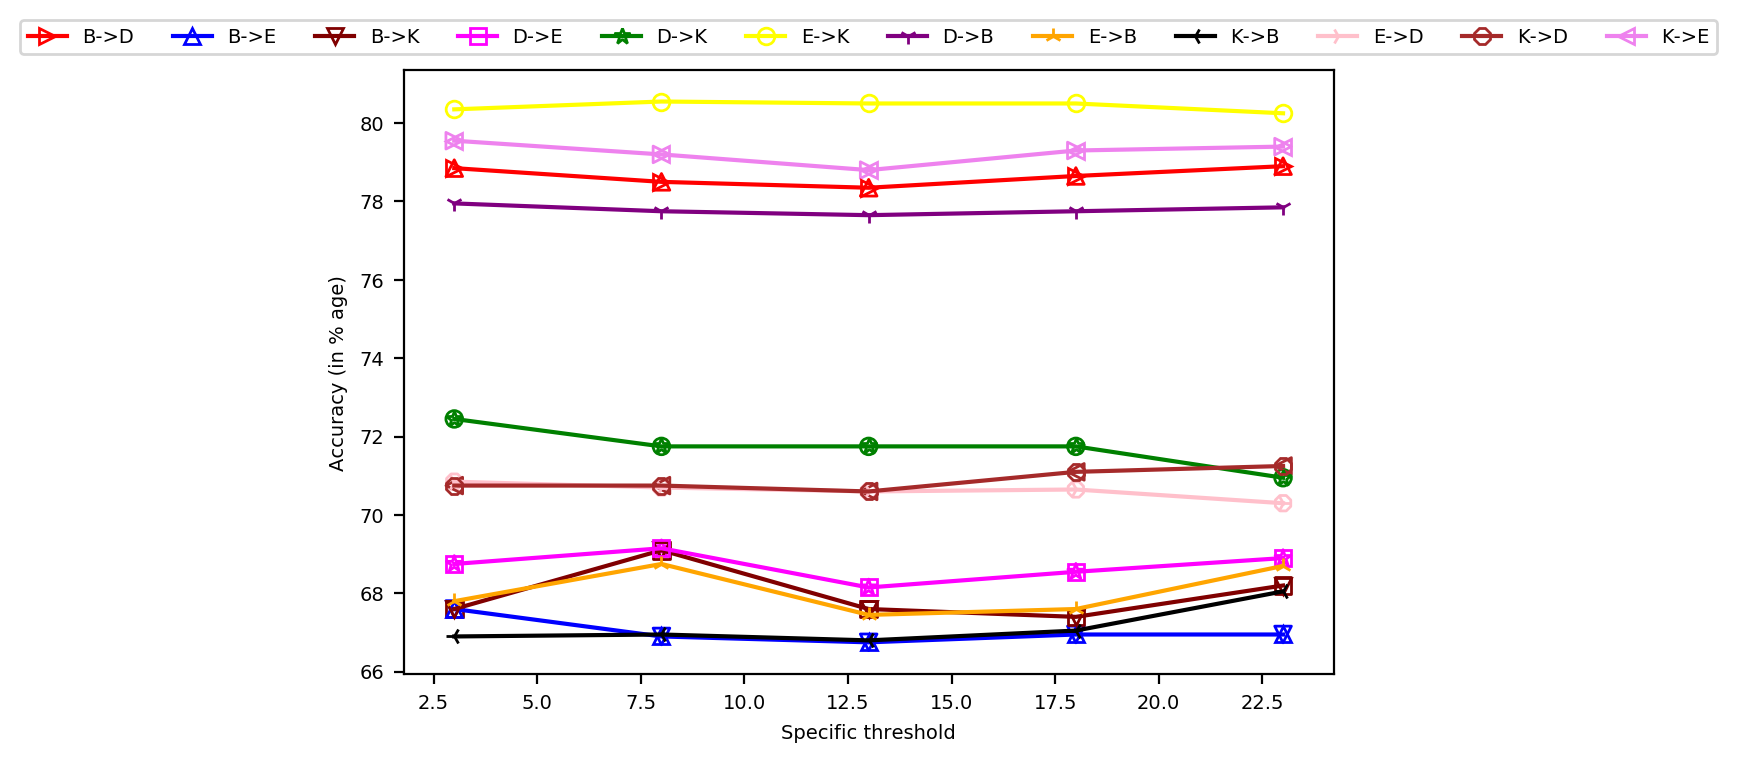
\includegraphics[width=1.1\textwidth]{m3s.png}
\figcaption{\emph { Accuracy(best) vs Specific Threshold}}}

\myfigure{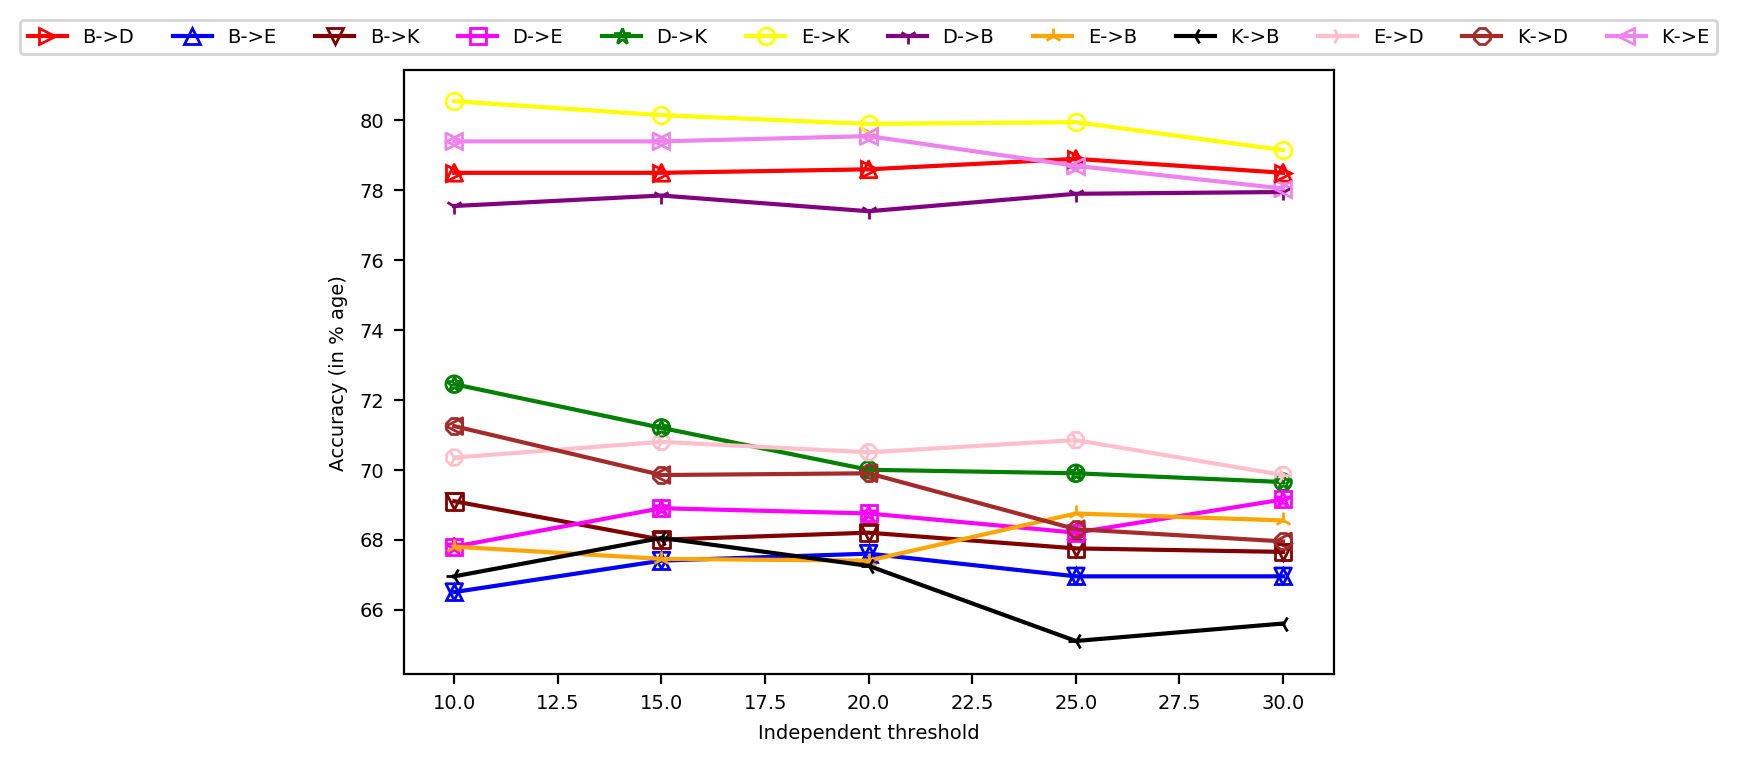
\includegraphics[width=1.1\textwidth]{m3i.png}
\figcaption{\emph { Accuracy(best) vs Independent Threshold}}}\newpage

\section{Methods Comparison}

\myfigure{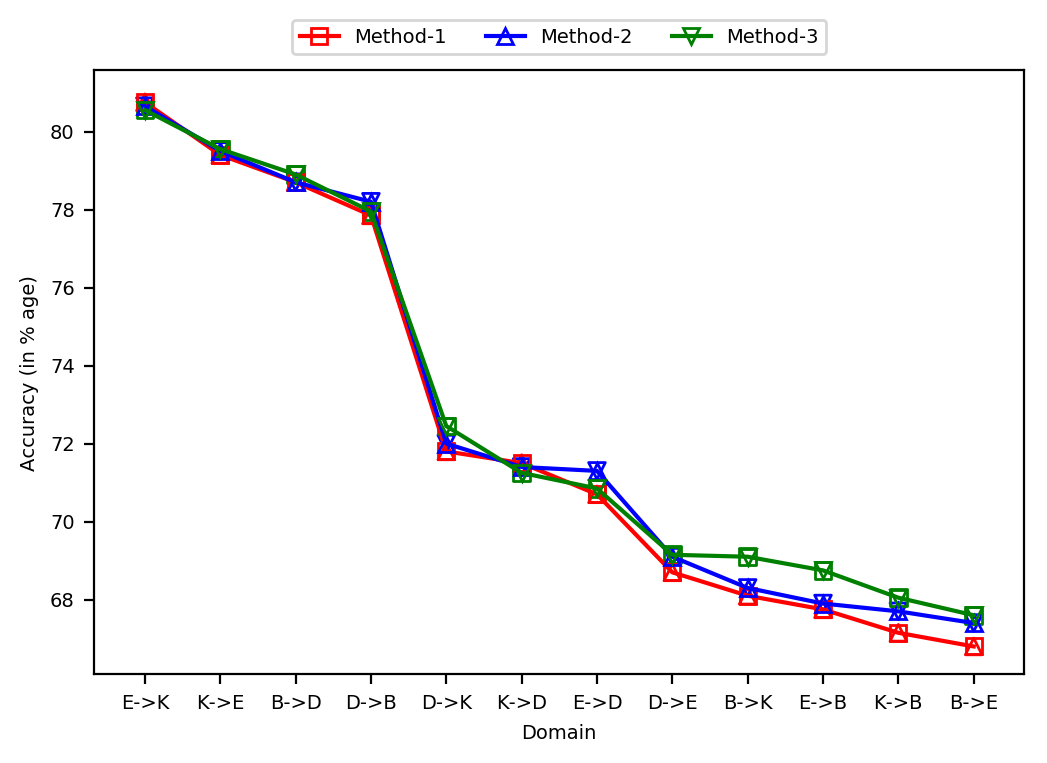
\includegraphics[width=1.1\textwidth]{all.png}
\figcaption{\emph { Accuracy(best) of each domain pair for all methods}}}



%-------------------------------------------------------------------------------

\chapter{Observations :}
\begin{enumerate}[label=\Roman*.]
\item After testing our methods with different combinations of domains(i.e Books \(\rightarrow\) Dvds, Dvds \(\rightarrow\) electronics.etc) we observed that : 
\begin{itemize}[label=$\diamond$]
\item For Model 1 :
\begin{enumerate}[label=\arabic*.]
\item We are obtaining best accuracy for various combinations of domains when the number of clusters lie in the range 25-30(Fig-9.1 ).
\item When specific threshold lies between 20-25, we get the best accuracy for given domains(Fig-9.2).
\item When independent threshold lies between 10-15 \& 23-28, the best accuracy is obtained for given combinations of domains(Fig-9.3).
\end{enumerate}

\item For Model 2 :
\begin{enumerate}[label=\arabic*.]
\item As evident from Fig-9.4 , we get best accuracy when mutual information based specific percentage cuttoff is the range 12.5\( \% \) \-33 \( \% \).
\item The optimum independent threshold lies between 10-15 and 20-25 (Fig-9.6).
\item The optimum cluster length lies between 20-30 (Fig-9.4).
\end{enumerate}

\item For Model 3 :
\begin{enumerate}[label=\arabic*.]
\item As evident from Fig-9.8 , we get best accuracy when mutual information based specific percentage cuttoff is the range 4\(\%\)-12.5\(\%\).
\item The optimum independent threshold lies between 10-20 (Fig-9.9).
\item The optimum cluster length lies between 20-30 (Fig-9.7).
\end{enumerate}
\end{itemize}

\item From table(Table-8.4), it can be observed that method 3 has best accuracy for 8 out of 12 combinations of domains though the difference between the accuracies is quite less.

\item As observed in Fig-9.1 to 9.9, there is a significant gap between accuracies of some combination of domains.
\end{enumerate}



%-------------------------------------------------------------------------

\chapter{Conclusions}
\begin{enumerate}[label=(\roman*)]
\item More related are the domains, more is the accuracy. for instance Books and Dvds (78\(\%\) ) are more related to each other than books and eletronics therefore they have better accuracy than books and electronics (67\(\%\)). This explains the gap between accurancies for some combination of domains in fig.
\item The best method for cross domain sentiment analysis on given dataset is Method 3 as it giving best results for 8 out of 12 combinations of domains.
\item The optimum cluster length always remains in range 20-30 irrespective of which method is used.
\item The optimum mutual information based specific percentage cuttoff drops from 12.5\(\%\) - 33\(\%\) to 4.5\(\%\) - 12.5\(\%\) when we shift from method 2 to method 3 respectively.
\end{enumerate}
%---------------------------------------------------------------------------------------------------
\begin{comment}
\chapter{Future Work}
\begin{enumerate}[label=\arabic*)]
\item Cleaning of datasets and preparing it for training and testing of our model.
\item Implementing proposed algorithm(SFA) and building our model with help of it.
\item Calculation of accuracy and selection of appropriate hyper parameters for optimal results.
\item Comparing our results with results of conventional methods used for cross domain sentimental analysis(e.g. Use of CNN).
\end{enumerate}
\end{comment}

\chapter{Softwares Used :}
Spyder 3 (Scientific PYthon Development EnviRonment)
\section{Language Used :}
Python 3.5
\section{Libraries Used :}
\begin{itemize}[label=$\circ$]
\item pandas (Python Data Analysis Library) for inputting the Dataset.
\item NumPy for creating the co-occurence matrix (i.e. a large multi-dimensional matrix).
\item The module pyplot of matplotlib library is used for graph plotting
re library for the usage of Regular Expressions for text cleaning.

\item Stopwords list from the ‘corpus’ package of nltk (Natural Language Processing Toolkit) data package.

\item PorterStemmer algorithm from the package nltk.stem.porter for stemming of words.

\item CountVectorizer class from sklearn.feature\_extraction.text submodule for building the matrix (sparse) of word counts from text documents.

\item TfidfTransformer class from sklearn.feature\_extraction.text submodule to convert the count matrix (sparse) to a matrix of TF\_IDF features.
\item SpectralClustering class from sklearn.cluster module for the Spectral Clustering of the bipartite graph (represented as the co-occurence matrix).
\item train\_test\_split function from sklearn.cross\_validation module for splitting the whole Dataset into random train and test sunsets.

\item SVC class from sklearn.svm module for classification of the test set.
\end{itemize}
 

\bibliographystyle{IEEEtran}
\bibliography{references}
\end{document}